\chapter{Annexes chapitre 4}
\section{Simulations hydrodynamiques et prise en compte de la pré-impulsion}
\label{an:4-FLASH_to_Smilei}

Dans le cadre de l'interaction d'un laser intense avec de la matière, l'émission spontanée présente dans la chaîne laser peut produire une pré-impulsion (voir chapitre \ref{chap:2-laser}) qui peut ioniser la cible et produire un pré-plasma avant l'arrivée de l'impulsion principale (voir chapitre \ref{chap:2-laser} et figure \ref{fig:A4-contraste_laser}). Ce pré-plasma peut modifier considérablement la physique de l'interaction de l'impulsion principale avec la cible (voir e.g. \parencite{chopineau_2019}). L'effet de cette pré-impulsion n'a pas été considéré dans les études menées au chapitre \ref{chap:6-opti_numerique}, mais le chaînage de codes permettant de l'étudier a néanmoins été développé dans le cadre de cette thèse.

\begin{figure}[htbp]
    \centering
    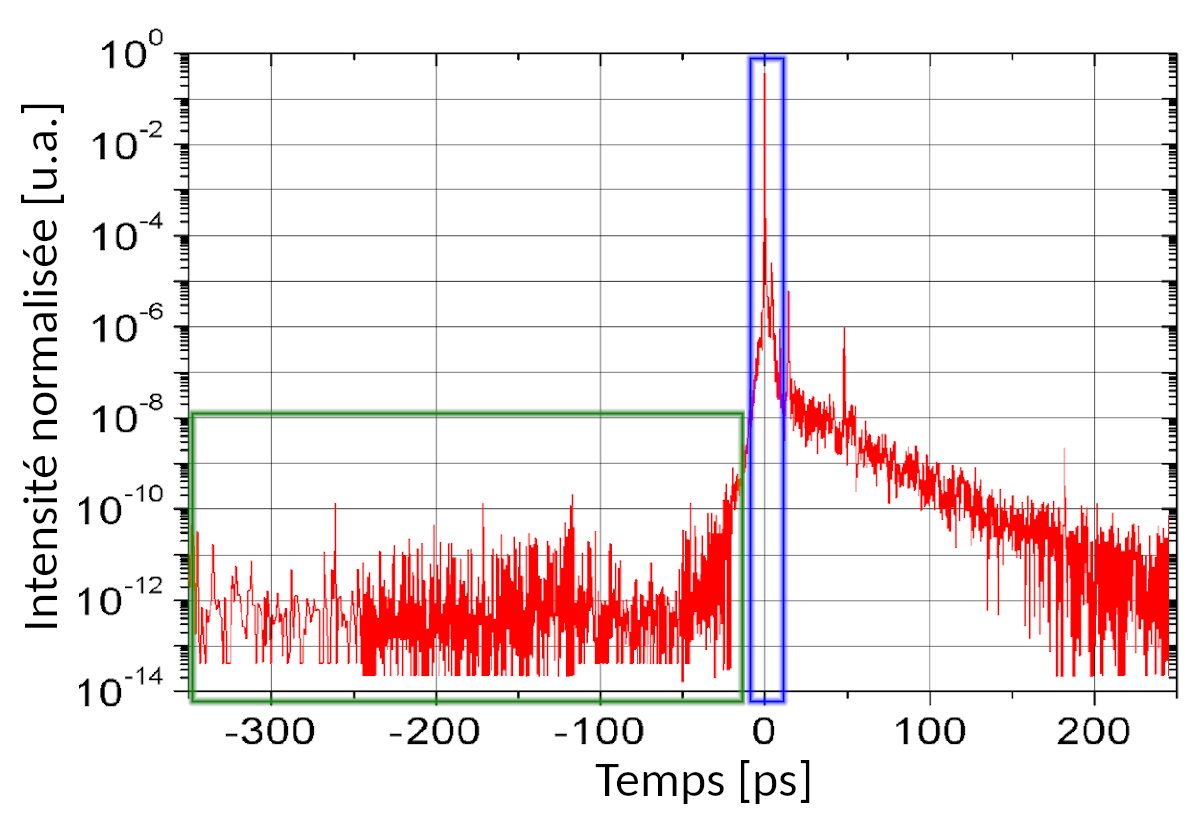
\includegraphics[width=0.6\linewidth]{2-laser/contraste_laser_Papadopoulos.png}
    \caption{Illustration du concept de contraste laser, pour la configuration du laser Apollon. L'impulsion principale est contenue dans l'encadré bleu, au temps 0, et son intensité est normalisée par sa valeur maximale. On observe dans l'encadré vert que plusieurs centaines de picosecondes avant l'arrivée de l'impulsion principale, le laser a une intensité non nulle, qui est ici de l'ordre de $10^{-12}$ fois sa valeur maximale. Une montée de l'intensité s'effectue rapidement quelques dizaines de picosecondes avant l'arrivée de l'impulsion principale. Image adaptée depuis \parencite{papadopoulos_2017}.}
    \label{fig:A4-contraste_laser}
\end{figure}

Comme nous avons pu le noter au chapitre \ref{chap:4-methodes_simu}, les codes de type Particle-In-Cell reposent sur la description du mouvement de macro-particules en interaction électromagnétique dans une grille fixe, ce qui leur permet d'être précis sur des simulations aux temps courts (typiquement moins de quelques dizaines de ps dans le cadre de l'interaction laser-solide). Néanmoins, ce type de code n'est pas compatible avec la simulation de la pré-impulsion, qui s'étend sur une durée de l'ordre de la nano-seconde \parencite{thaury_2007}. Ainsi, ce type de simulations est typiquement effectuée à l'aide de codes hydrodynamiques, tel que FLASH par exemple \parencite{fryxell_2000}, qui décrit cette fois-ci non pas des macro-particules en interaction, mais des quantités macroscopiques locales telles que des profils de températures, de vitesse, de densité ou de degrés d'ionisation par exemple. 

Dans le code Smilei, l'initialisation de l'état du plasma s'effectue à l'aide d'un fichier d'entrée en Python, et les caractéristiques (positions et impulsions) des macro-particules sont générées à partir de ces mêmes quantités macroscopiques locales. Ainsi, il est possible de simuler l'interaction de la pré-impulsion (encadré vert de la figure \ref{fig:A4-contraste_laser}) avec la cible à l'aide du code FLASH, puis de récupérer l'état du plasma pour l'injecter dans le code Smilei afin de simuler l'interaction de l'impulsion principale (encadré bleu de la figure \ref{fig:A4-contraste_laser}) avec le plasma produit ainsi que l'accélération d'électrons.

Pour ce faire, il est nécessaire de définir chacune de ces quantités en tout point de la grille PIC. Cependant, les grilles spatio-temporelles des simulations FLASH et Smilei n'ont a priori pas de raison d'être identiques, et il faut donc procéder à une interpolation des profils des quantités hydrodynamiques sur la grille PIC.
Cette opération peut être effectuée notamment grâce à la méthode \texttt{griddata} du module \texttt{scipy}. Deux difficultés se présentent néanmoins lors de cette opération :
\begin{itemize}
    \item Tout d'abord, l'initialisation des profils (densité, température, ...) doit être effectuée avec précautions. En effet, celle-ci doit être effectuée dans les blocs \texttt{Species} à l'aide d'une fonction Python retournant la valeur du profil considéré à une position donnée (position $(x,y)$ en 2D plan par exemple). Néanmoins, si l'interpolation est réalisée dans cette fonction Python, l'initialisation du code peut prendre beaucoup de temps (avec Smilei v4.5 du moins). 
    Une solution pour contourner le problème peut être de calculer et sauvegarder les différents profils sur les points de la grille PIC dans des matrices \texttt{numpy} hors du bloc \texttt{Species}, puis de lire ces valeurs de profils via une fonction Python dans les blocs \texttt{Species}. 
    Il est à ce titre intéressant de noter que la valeur d'un profil donné à la position $(x,y)$ peut être retrouvé à l'indice $(i,j)$ de la matrice de profil précédemment calculée, où $i$ est la valeur entière de $x/dx$ avec $dx$ la taille de maille selon $x$, et $j$ est la valeur entière de $y/dy$ avec $dy$ la taille de maille selon $y$.
    
    \item La gestion du degré d'ionisation doit aussi faire l'objet d'une attention particulière. En effet, dans le code FLASH le degré d'ionisation est une valeur moyenne locale, qui peut prendre n'importe quelle valeur réelle inférieure ou égale au numéro atomique des atomes en présence. Au contraire, dans le code Smilei le degré d'ionisation d'un macro-ion ne peut prendre que des valeurs entières. Le degré d'ionisation local dans une maille donnée est néanmoins une valeur moyenne qui peut éventuellement prendre une valeur non entière (e.g. une maille contenant deux macro-ions de degré d'ionisation respectivement 1 et 2 aura un degré d'ionisation local de $1.5$). Pour chaque maille, le nombre de macro-ions doit donc être suffisamment élevé pour permettre de correctement représenter le degré d'ionisation du profil d'entrée. Ainsi, pour avoir un nombre de particules par mailles raisonnable dans le code PIC, il est nécessaire d'effectuer un arrondi sur les valeurs des profils de degré d'ionisation du code FLASH, afin de correctement représenter le degré d'ionisation local du plasma (un arrondi entier sur le profil d'ionisation FLASH permet de le représenter correctement dans Smilei avec une seule particule par maille, un arrondi à la première décimale à l'aide de 10 particules par maille, un arrondi à la deuxième décimale à l'aide de 100 particules par maille, etc ...). Pour conserver la quasi-neutralité locale du plasma, le profil de densité électronique peut aussi être re-calculé à partir du profil de degré d'ionisation arrondi ainsi que du profil de densité ionique (i.e. $n_e = Z^* ~  n_i$, avec $n_e$ la densité électronique, $Z^*$ le degré d'ionisation et $n_i$ la densité ionique).
\end{itemize}

Ces développements ont été menés en collaboration avec J. Bonvalet, et ont fait l'objet d'une très précieuse aide de l'équipe de Smilei, notamment via les \textit{issues} \href{https://github.com/SmileiPIC/Smilei/issues/129}{129} et \href{https://github.com/SmileiPIC/Smilei/issues/180}{180} de leur dépot github.

\chapter{Annexes chapitre 5}
\section{Section efficace intégrée pour la somme de deux fonctions simples}
\label{an:5-somme_2_fonctions}

Dans le chapitre \ref{chap:5-opti_theorique}, nous avons donné une méthode permettant de calculer la section efficace intégrée pour des fonctions pouvant être exprimées sous la forme :
\begin{equation}
    f_i(E_i, K_i) = \dfrac{g_i(E_i/K_i)}{K_i} \rm ,
    \label{eq:A5-definition_g}
\end{equation}
et satisfaisant
\begin{equation}
    \int_0^{+\infty} f_i (E_i, K_i) ~ dE_i = \int_0^{+\infty} g_i (E_i/K_i) ~ d(E_i/K_i) = 1 \rm ,
    \label{eq:A5-normalisation_g}
\end{equation}

Sous ces conditions, la définition de la section efficace intégrée :
\begin{equation}
    \sigma_{\gamma\gamma}^{int} = \iint_{0}^{+\infty} f_1 ~ f_2 ~ \sigma_{\gamma\gamma} ~ dE_1 ~ dE_2 \rm ,
    \label{eq:A5-sigma_int_definition}
\end{equation}
pouvait être réduite à une fonction d'une seule variable :
\begin{equation}
    \sigma_{\gamma\gamma}^{int}(\zeta) = \dfrac{1}{\zeta} \int_0^{+\infty} g_2(\eta/\zeta) \left[\dfrac{1}{\eta} \int_0^{+\infty} g_1(s/\eta) \sigma_{\gamma\gamma}(s) ds \right] d\eta ~ \rm .
    \label{eq:A5-sigma_int_1_variable}
\end{equation}

Cette fonction pouvait de plus être ajustée avec une fonction d'ajustement, nommée $h$. Celle-ci pourrait néanmoins aussi être utilisée pour calculer la section efficace intégrée avec des distributions en énergie étant une somme de fonctions de la forme \ref{eq:A5-definition_g}.

A titre d'illustration, considérons que la distribution en énergie du faisceau $1$ puisse être décrite par une fonction $f_1$ satisfaisant à la fois les équations (\ref{eq:A5-definition_g}) et (\ref{eq:A5-normalisation_g}), et que la distribution en énergie du faisceau $2$ puisse être exprimée par une fonction à deux composantes telle que :
\begin{equation}
    \tilde{f_2}(E_2, K_{2a}, K_{2b}) = p \times f_{2,a}(E_2,K_{2a}) + (1-p) \times f_{2b}(E_2,K_{2b}) ~ \rm ,
\end{equation}
où $K_{2a}$ et $K_{2b}$ sont deux énergies caractéristiques, $f_{2a}$ et $f_{2b}$ sont des fonctions qui satisfont les conditions (\ref{eq:A5-definition_g}) et (\ref{eq:A5-normalisation_g}), et $p \in[0,1]$ définit le poids relatif de chacune des composantes de la distribution en énergie $\tilde{f}_2$.
Ce type de distribution en énergie pourrait éventuellement être utilisé pour modéliser une distribution en énergie composé de deux exponentielles par exemple.

En insérant cette distribution en énergie dans la définition de la section efficace intégrée donnée par l'équation (\ref{eq:A5-sigma_int_definition}), on peut remarquer que $\sigma_{\gamma\gamma}^{int}$ peut s'exprimer comme une somme de deux termes, qui chacun d'entre eux peuvent se réduire à la forme de l'équation (\ref{eq:A5-sigma_int_1_variable}). Ainsi, chacun de ces termes peut être approximé par une fonction de la forme de $h$, et la section efficace intégrée résultante peut être estimée via :
\begin{equation}
    \sigma_{\gamma\gamma}^{int} \approx p \times h_{a}(\zeta_a) + (1-p) \times h_{b}(\zeta_b) ~ \rm ,
\end{equation}
où $h_a$ et $h_b$ sont les fonctions d'ajustement correspondant à l'interaction de la distribution en énergie du faisceau $1$ avec respectivement la première et la seconde composante de la distribution en énergie du faisceau $2$ ($f_{2a}$ et $f_{2b}$ respectivement), et où $\zeta_a=2 K_1 K_{2a} (1-\cos\psi_{12})$ et $\zeta_b=2 K_1 K_{2b} (1-\cos\psi_{12})$. 
Ce type d'approche pourrait être généralisé pour traiter des distributions en énergies plus complexes.

\chapter{Annexes chapitre 6}
\section{Données de simulations PIC}
\label{an:6-PIC}

\begin{figure}[h]
    \centering
    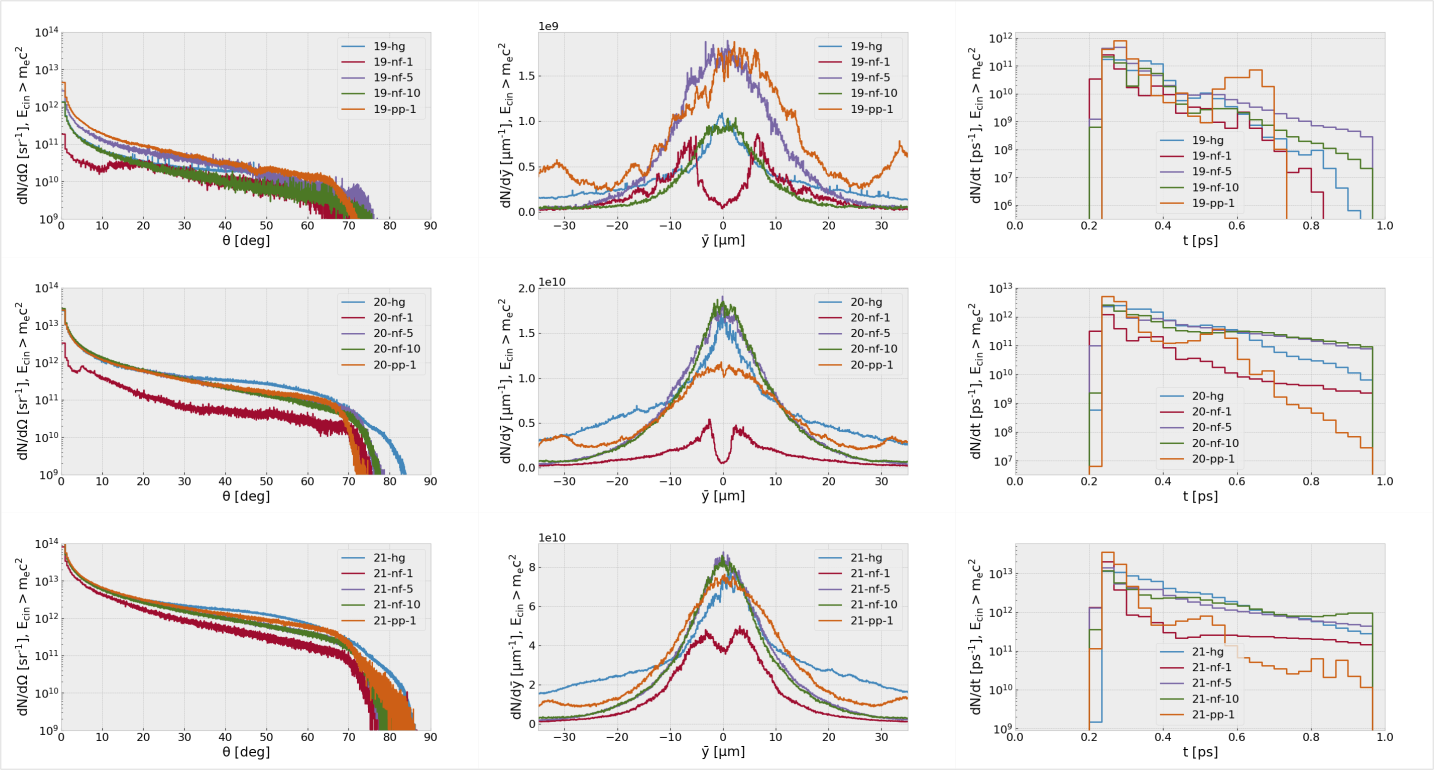
\includegraphics[width=\linewidth]{8-annexes/absorber_electron.png}
    \caption{Caractéristiques des sources d'électrons éjectées du substrat.}
\end{figure}

\newpage

\begin{figure}[h]
    \centering
    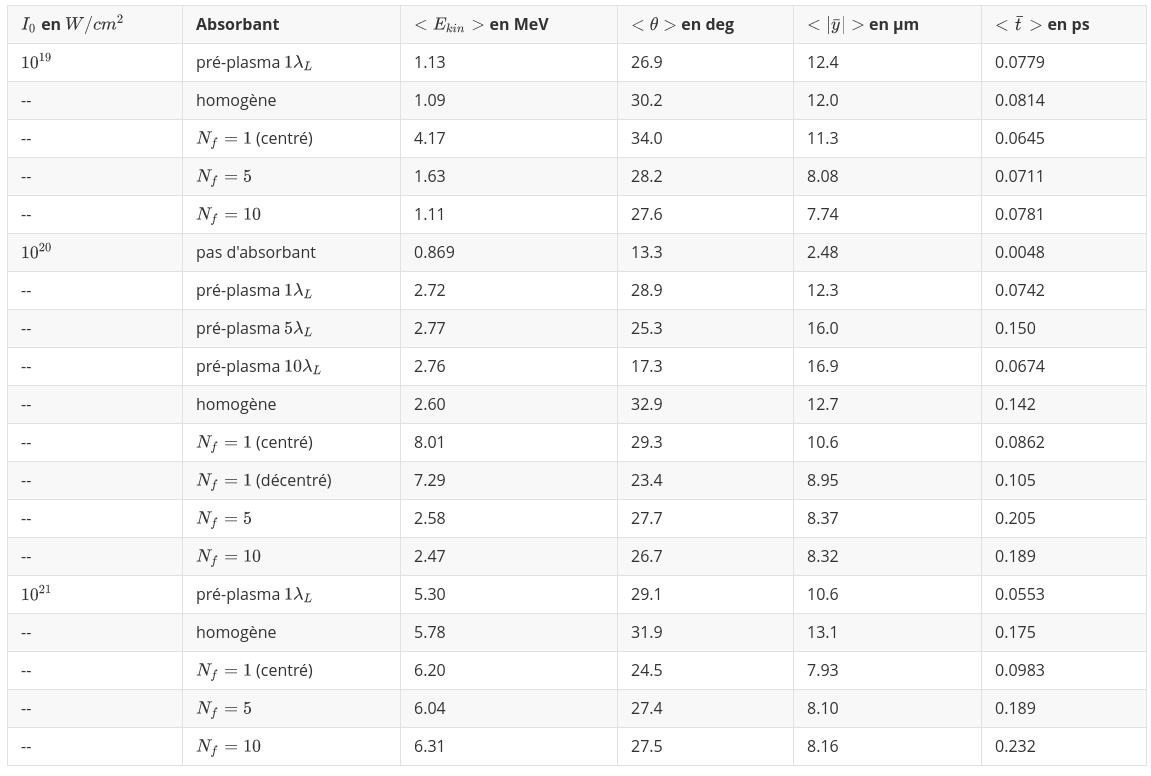
\includegraphics[width=\linewidth]{8-annexes/tableau_quantites_moyennes.png}
    \caption{Valeurs moyennes des différentes quantités, pour les électrons exportés avec une énergie cinétique $>m_e c^2$.}
\end{figure}

\newpage

\hspace{-2cm}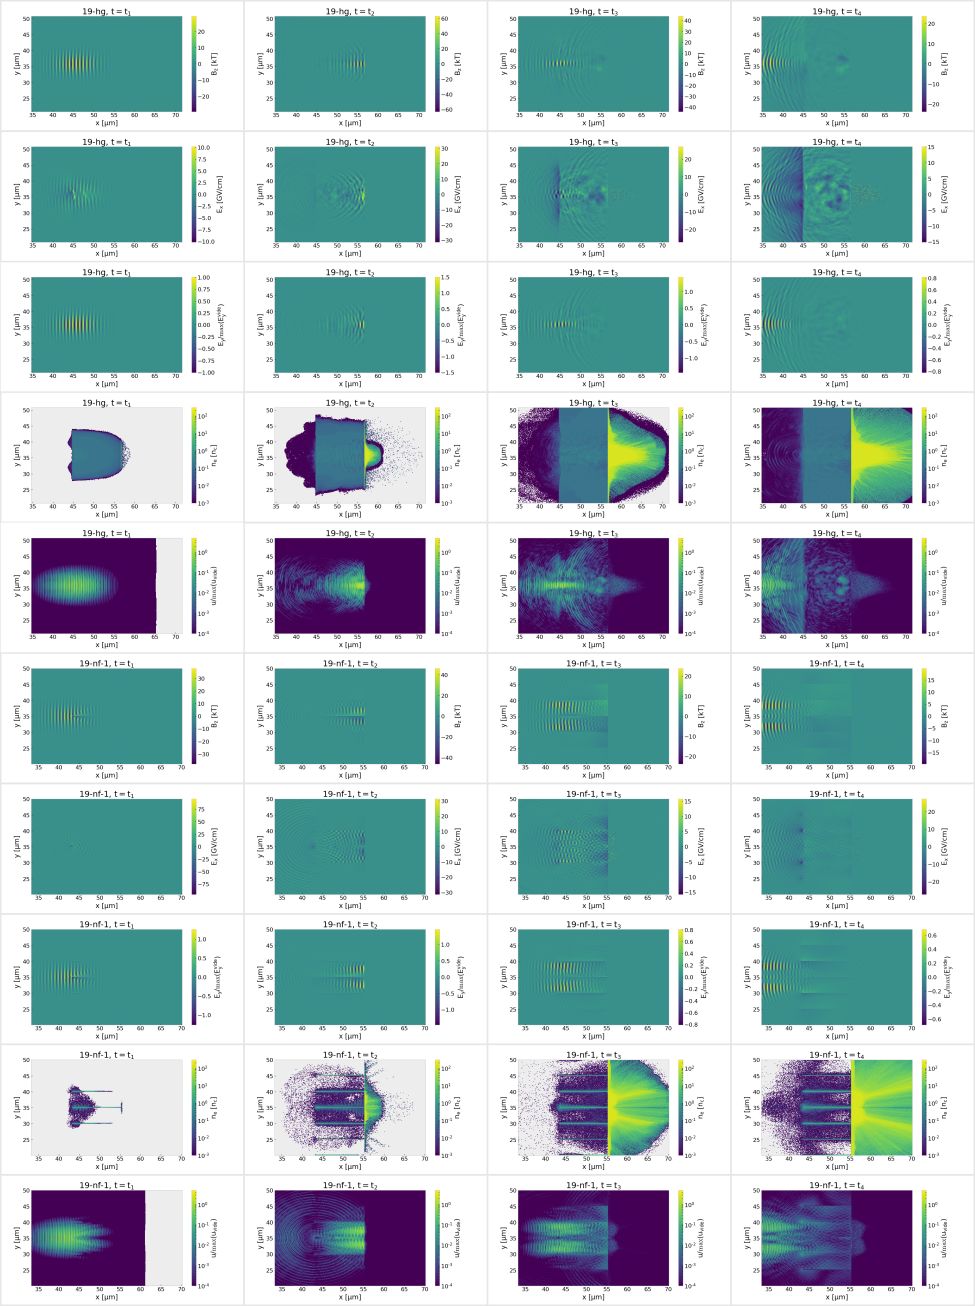
\includegraphics[width=1.2\linewidth]{8-annexes/absorber_19_p1.png}
\newpage

\hspace{-2cm}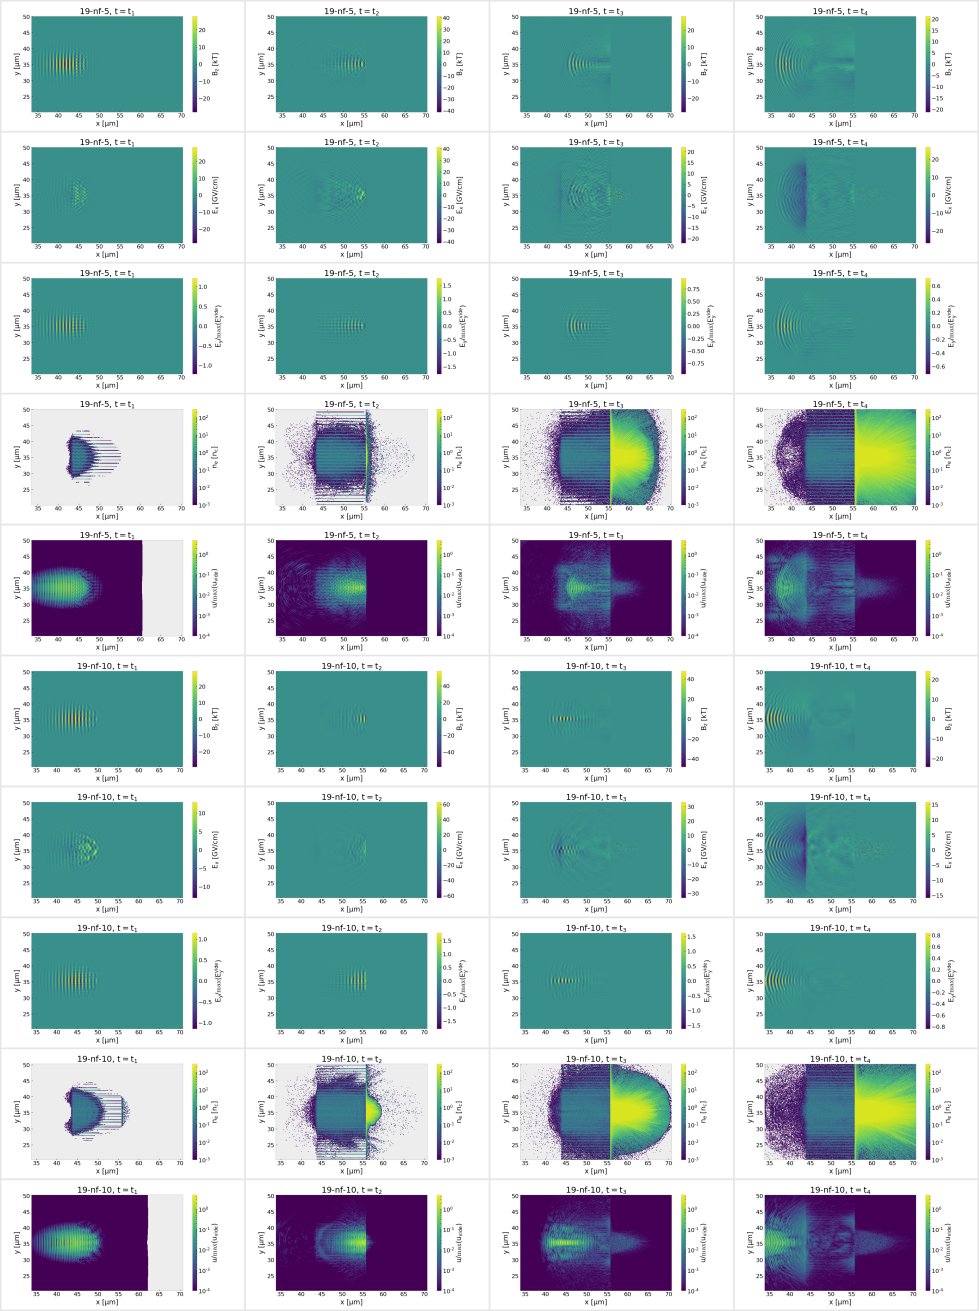
\includegraphics[width=1.2\linewidth]{8-annexes/absorber_19_p2.png}
\newpage

\hspace{-2cm}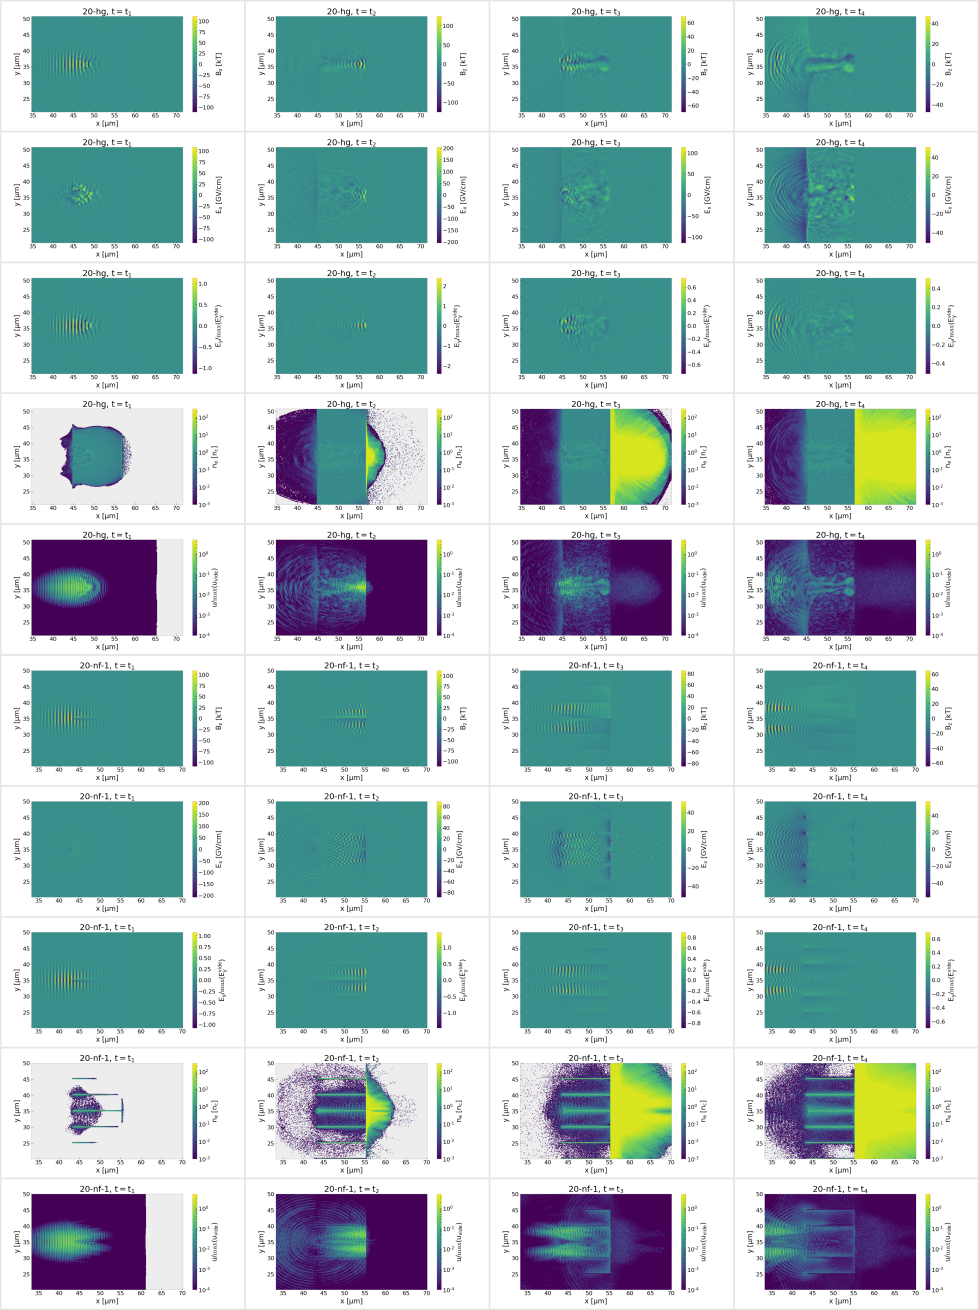
\includegraphics[width=1.2\linewidth]{8-annexes/absorber_20_p1.png}
\newpage

\hspace{-2cm}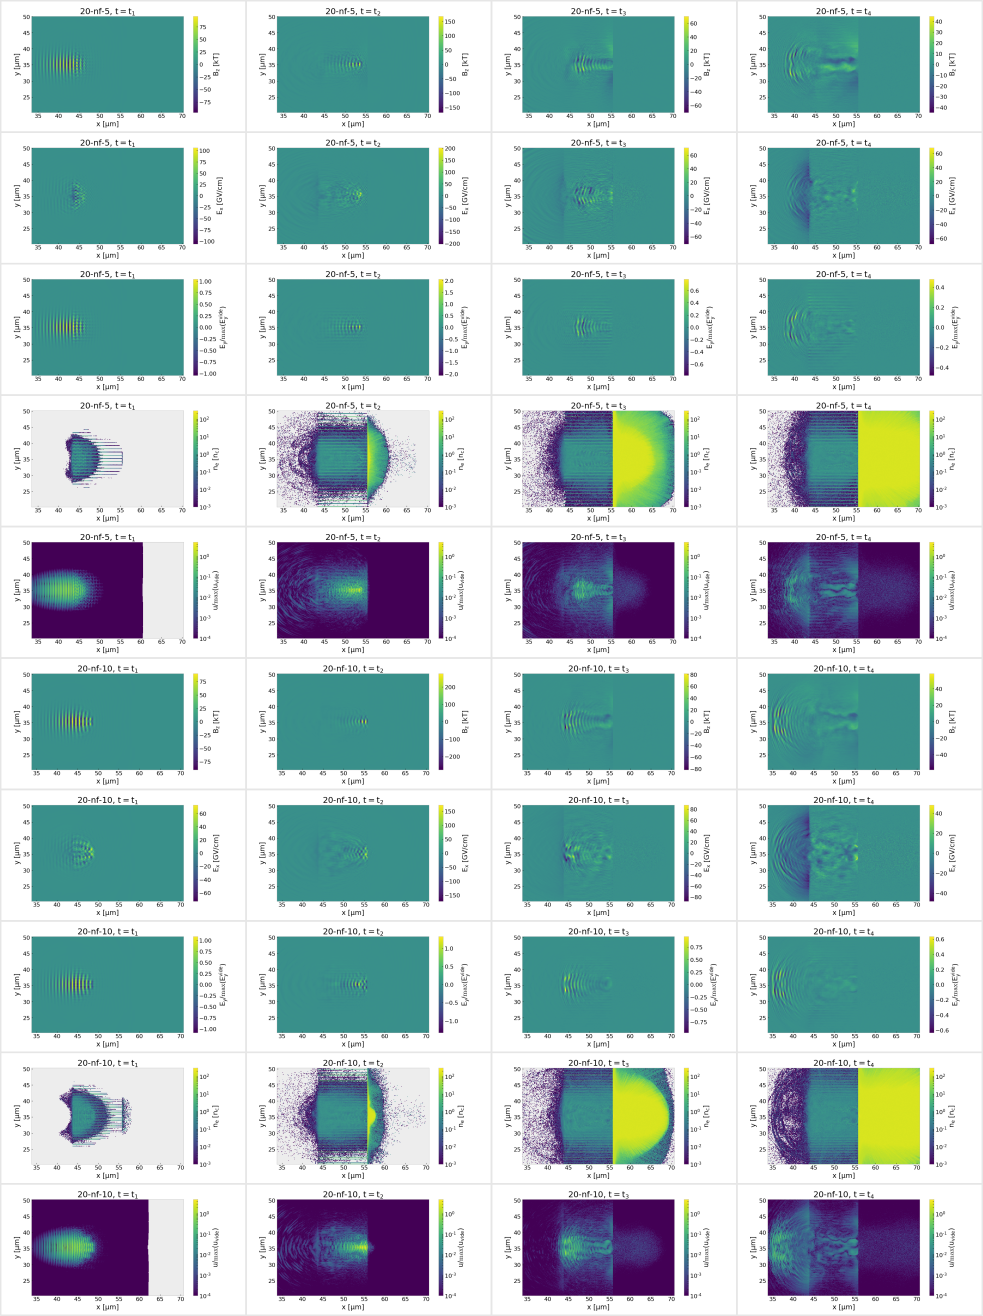
\includegraphics[width=1.2\linewidth]{8-annexes/absorber_20_p2.png}
\newpage

\hspace{-2cm}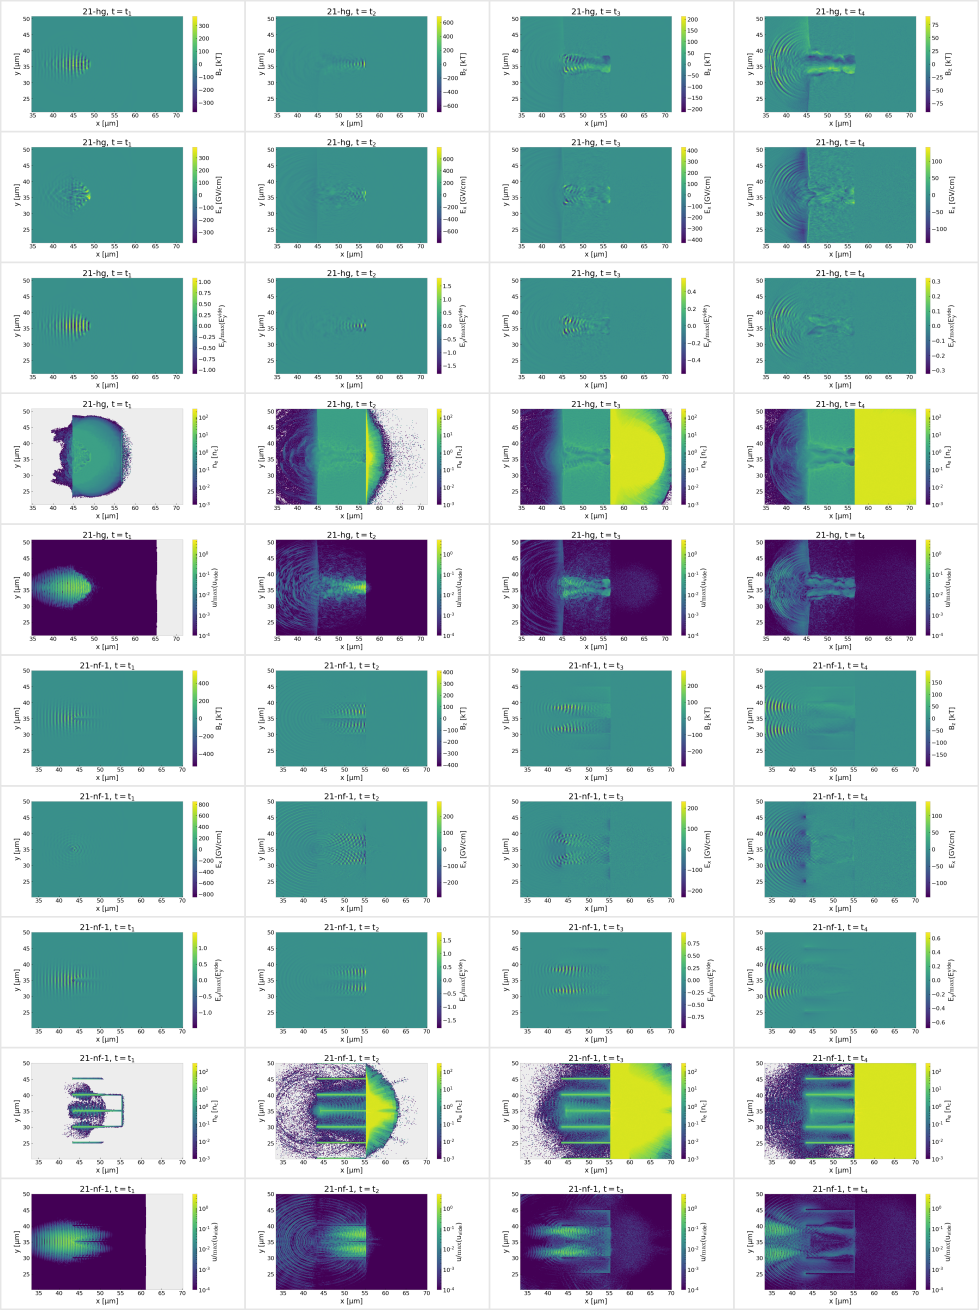
\includegraphics[width=1.2\linewidth]{8-annexes/absorber_21_p1.png}
\newpage

\hspace{-2cm}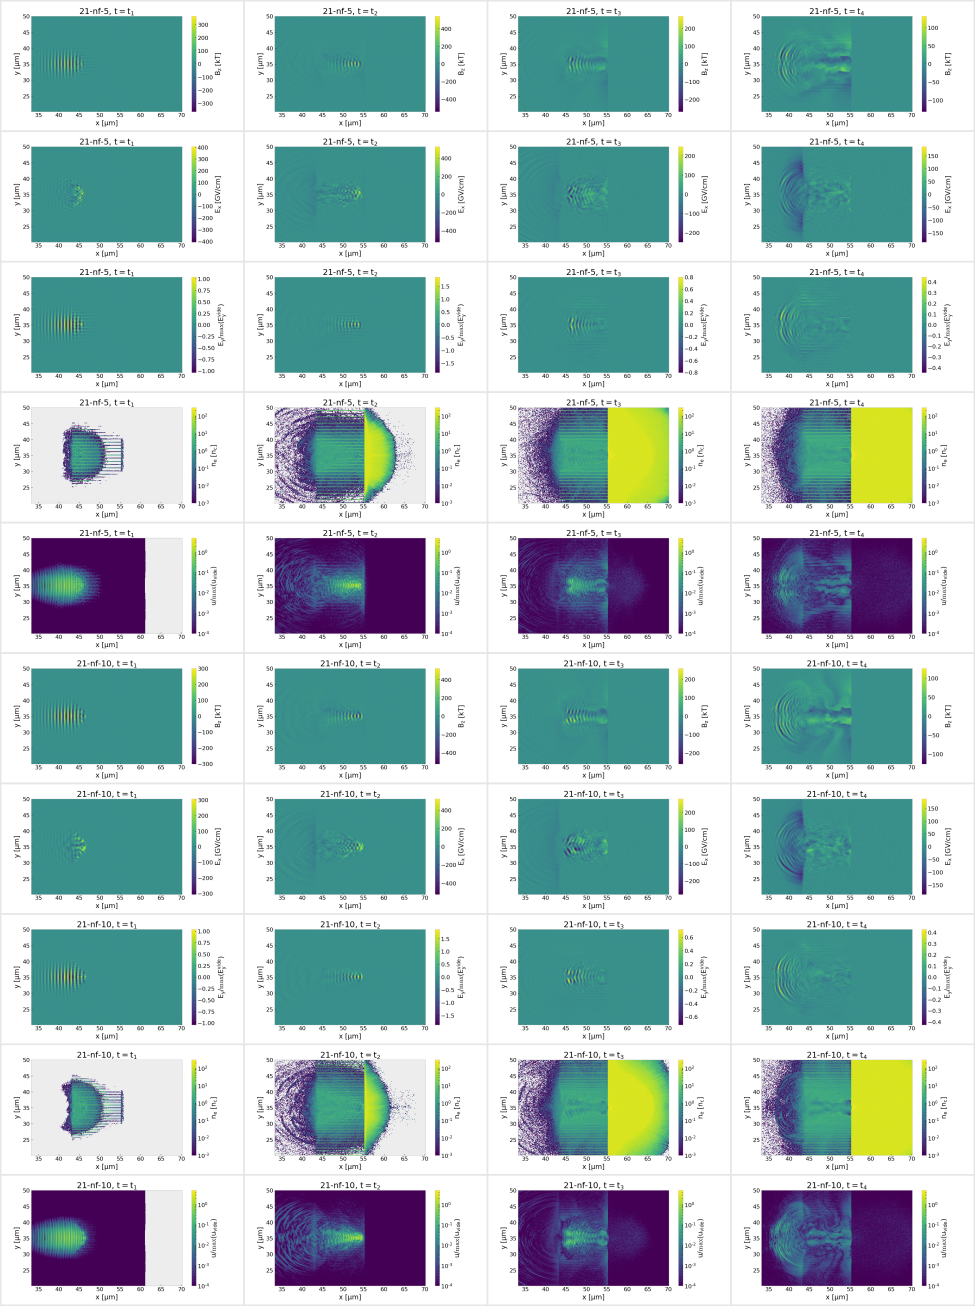
\includegraphics[width=1.2\linewidth]{8-annexes/absorber_21_p2.png}

\newpage
\newpage
\section{Données de simulations Monte Carlo}
\label{an:6-MC}

\begin{figure}[h]
    \centering
    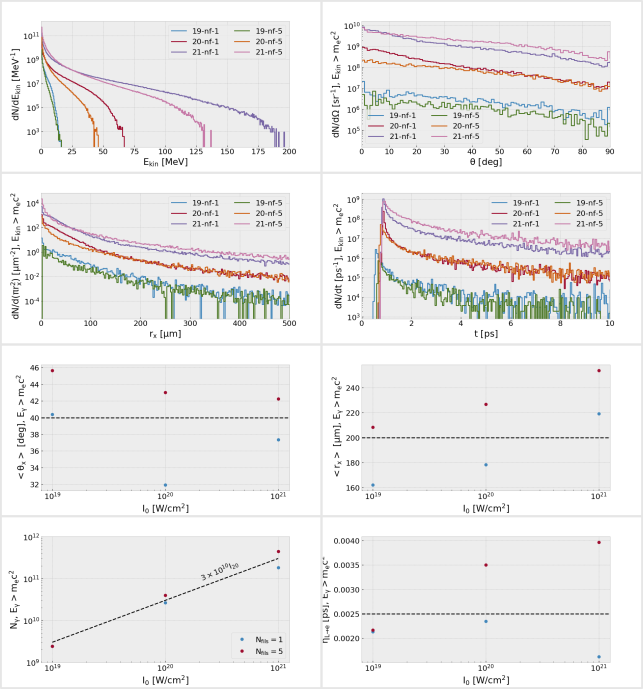
\includegraphics[width=\linewidth]{8-annexes/converter_gamma.png}
    \caption{Caractéristiques des sources de photons $\gamma$ obtenues par Bremsstrahlung, pour les particules d'énergies $>m_e c^2$}
\end{figure}
\newpage
\begin{figure}[h]
    \centering
    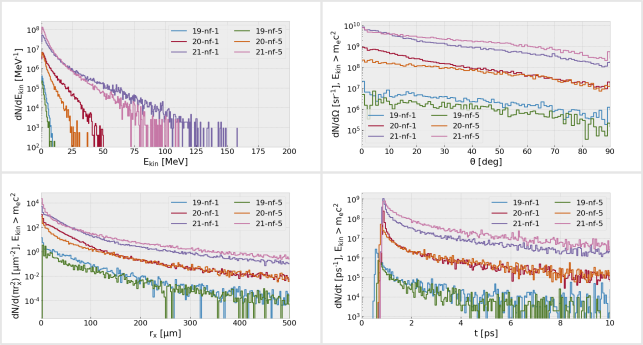
\includegraphics[width=\linewidth]{8-annexes/converter_positron.png}
    \caption{Caractéristiques des sources de positrons de bruit produites dans les sources Bremsstrahlung, pour les particules d'énergies $>m_e c^2$}
\end{figure}